\begin{figure}[th]
\centering
\subfigure[]{
    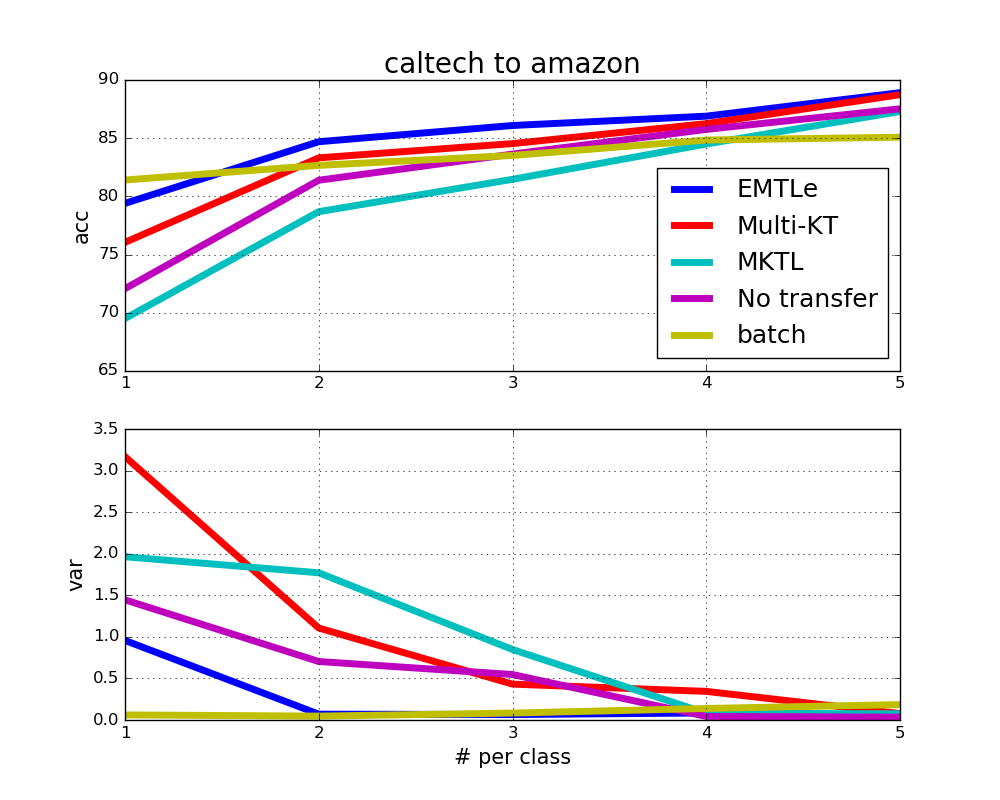
\includegraphics[width=0.25\textwidth]{fig/2caltechtoamazon.png}\label{a}
}
\subfigure[]{
    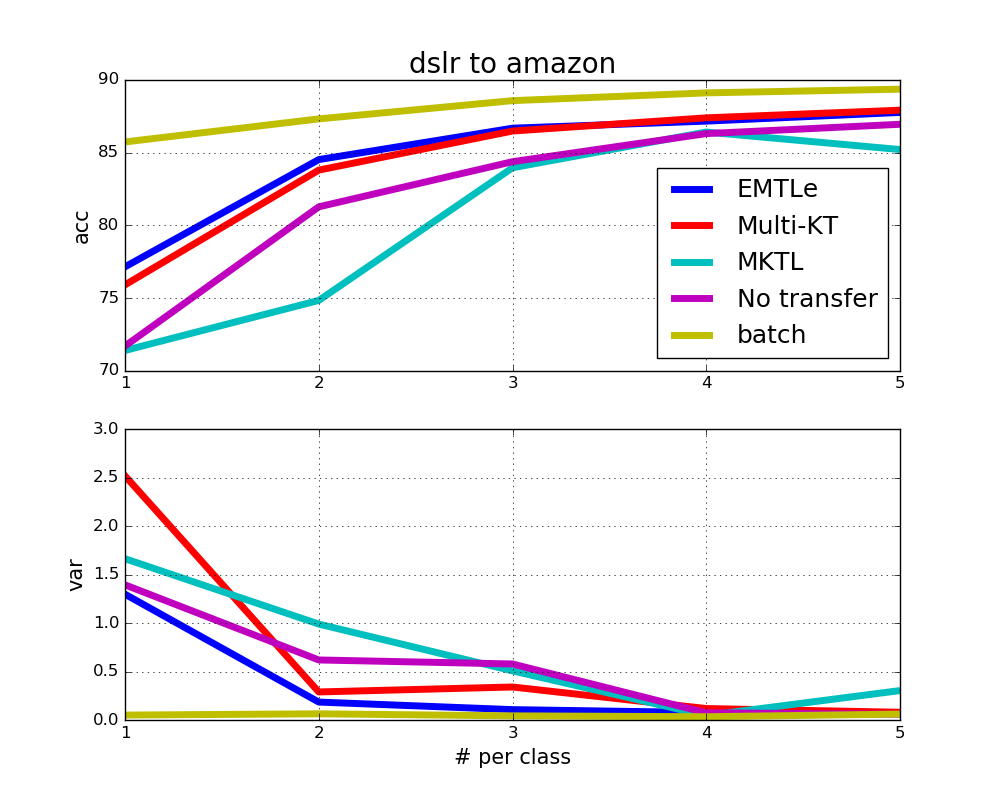
\includegraphics[width=0.25\textwidth]{fig/2dslrtoamazon.png}\label{b}
}
\subfigure[]{
	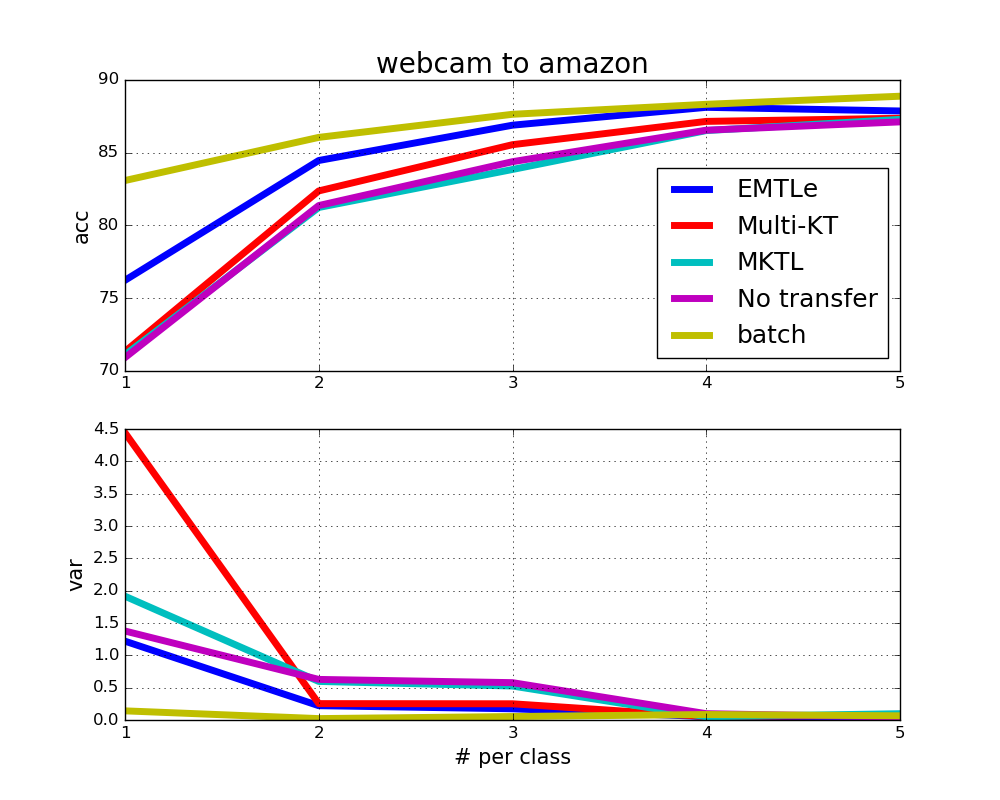
\includegraphics[width=0.25\textwidth]{fig/2webcamtoamazon.png}\label{c}
}\\
\subfigure[]{
	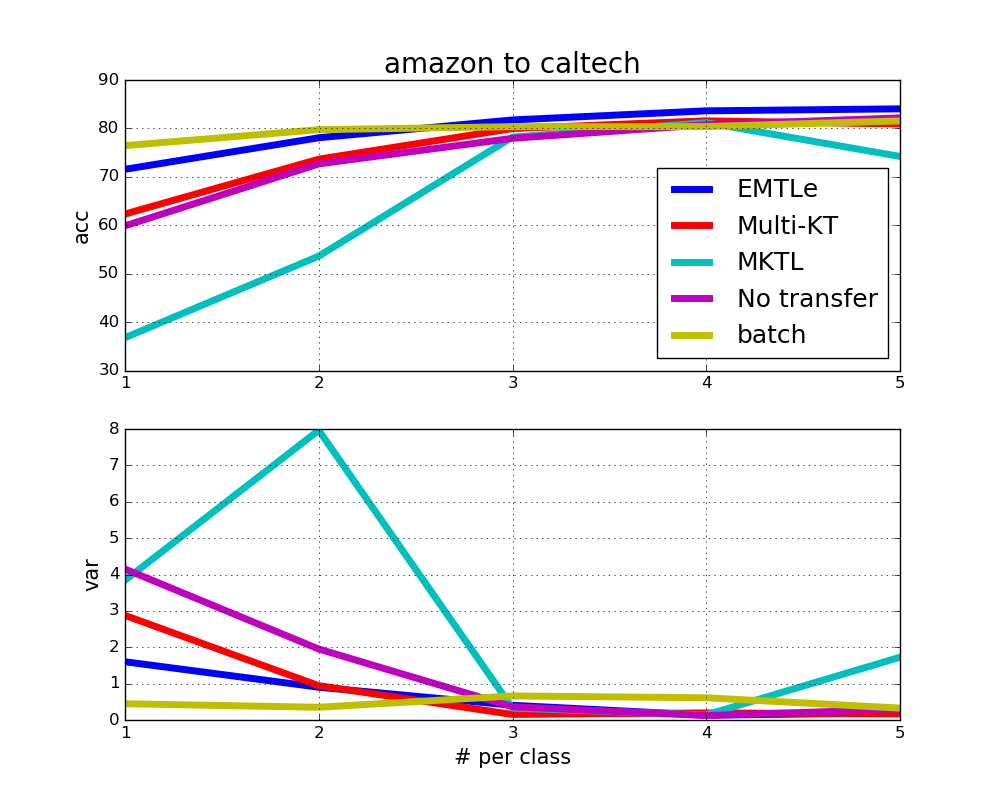
\includegraphics[width=0.25\textwidth]{fig/2amazontocaltech.png}\label{d}
}
\subfigure[]{
	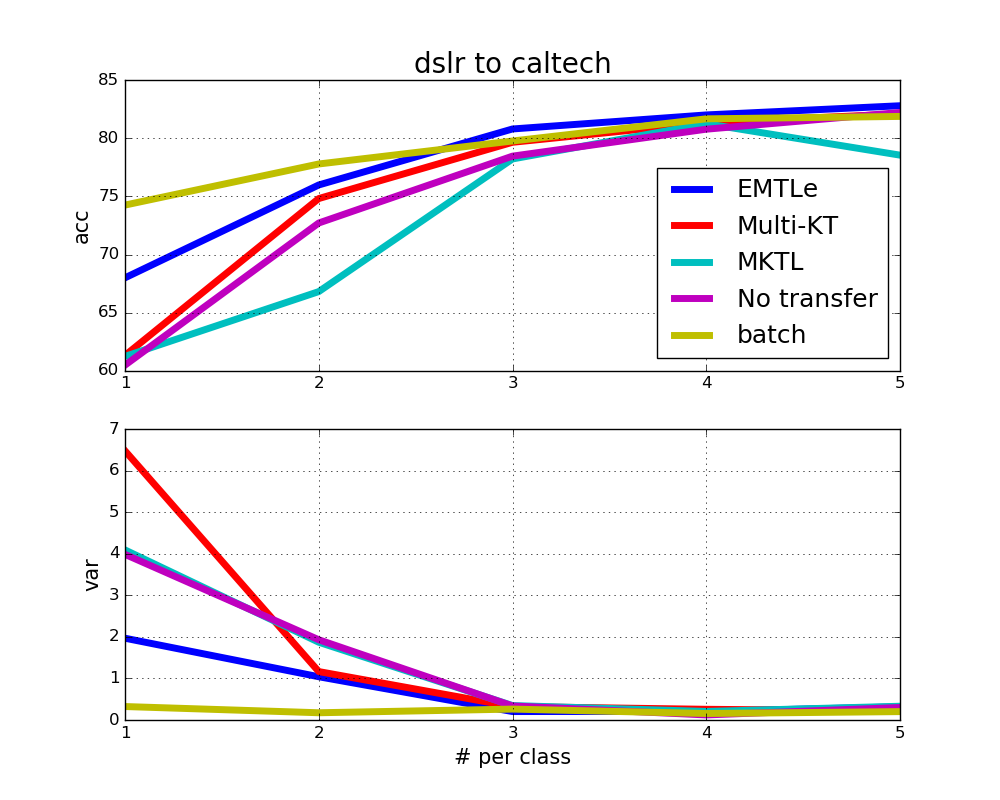
\includegraphics[width=0.25\textwidth]{fig/2dslrtocaltech.png}\label{e}
}
\subfigure[]{
	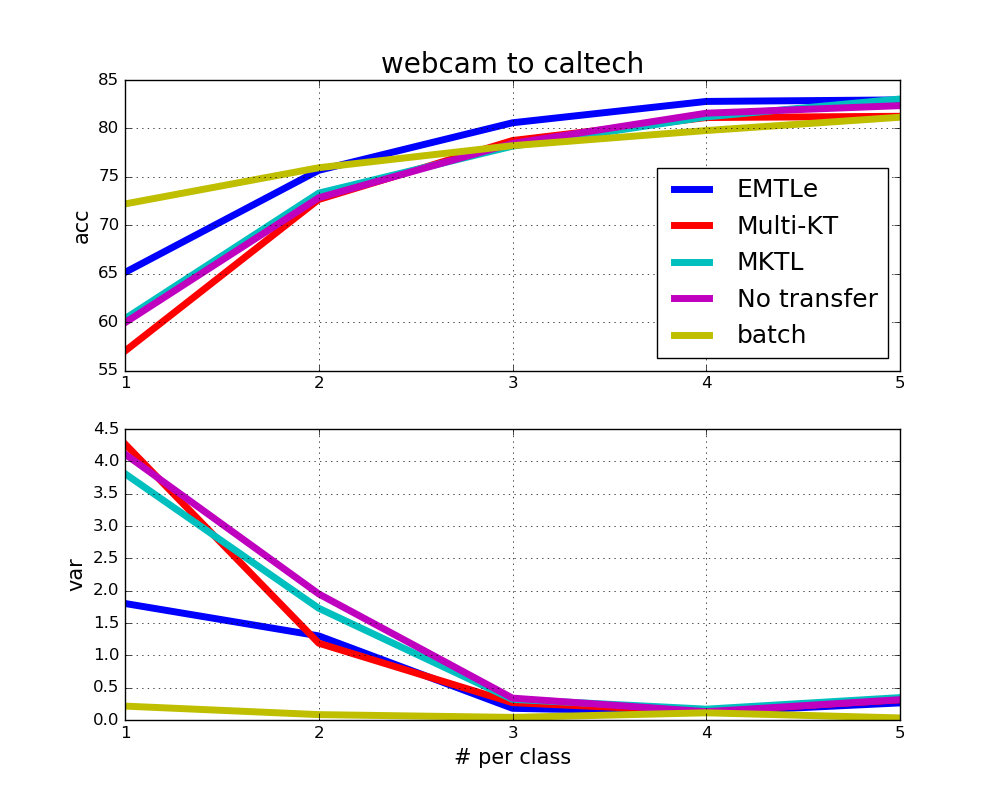
\includegraphics[width=0.25\textwidth]{fig/2webcamtocaltech.png}\label{f}
}\\
\caption{Recognition accuracy and variance for HTL domain adaptation using single type of the source classifier. 5 different sizes of target training sets are used in each group of experiments.}
\label{fig:exp}
\end{figure}

\textbf{Observation \& discussion:} EMTLe can significantly outperform other baselines especially when the training size is small. Moreover, we can see that compared to the other two transfer methods, EMTLe is the most stable method (low variance). As we have discussed above, without the $\ell_2$ penalty in the objective functions when the training set is small, these two HTL baselines could be prone to overfitting and not able to effectively exploit the source models.
As the training size increases, the variance of the data decreases. The advantage of the $\ell_2$ penalty term become less significant and all methods tend to show similar performance.
In some experiments, we can see that EMTLe can even outperform the Batch method which can access more information and is expected to outperform the other methods under the setting of HTL.